\clearpage

\section{EV Driver Interface}

The UI is one aspect of EVs or automobiles in general that often has not been the center of effort and discussion and used to play a minor role in development. However, in order to fully maximize an EV's potential and to ensure consumer adoption, the design and functionality of UI is an important aspect. Designers have also picked up on that topic \cite{driver-1}.

Due to reports from large user field studies, which show that newly developed interfaces can lead to distraction and confusion of drivers \cite{driver-2} \cite{driver-3}, it is important not to change industry standards completely or reinventing the wheel, but instead integrate new functionality within existing features. 

\subsection{UI Issues and Challenges within Electric Vehicles}

Drivers of electric vehicles will face new challenges unknown to them if they have been driving conventional automobiles before. The task of the EV's UI will be to guide the driver through those challenges while still providing a positive and rewarding experience.

The driver of electric vehicles will encounter major challenges quite quickly with electric vehicles today, such as the charging procedures, or even a route that differs from his usual driving routine because it is more energy efficient or due to the fact that it is the route that was calculated by the scheduling algorithm for charging stops.

The task of the UI is therefore also to teach and guide the driver through the process, while still keeping up the driving pleasure and not making that trip a frustrating experience. While an unexperienced EV driver will and probably wants more guidance about recharging duration, charging procedures, etc., an experienced driver probably needs less guidance and information and will even find too much guidance obstructing.

Furthermore, an electric vehicle behaves quite differently compared to a conventional car due to its special characteristics. It has a much more limited driving range, higher acceleration performance, lower top speed and due to the large battery, a higher car weight and limited interior space.

Therefore, those factors also need to be acknowledged when designing an UI in order to make a driver aware of limitations, and potentially warn him or send notifications to inform him. 

Battery technology today only allows for a limited range in comparison to conventional cars. Depending on design and size, the range is below 250km, which is usually sufficient for most trips (\cite{driver-4} 80\% with Mini-E, \cite{driver-8} 95\% with a range of 100 miles) and is usually even enough for daily use \cite{driver-5} \cite{driver-6}. But when it comes to a larger trip today, a driver is often faced with the challenge of planning the perfect route, with charging stops that are also not already blocked at the time of his arrival.

That is where our UI will step in, so that the driver can just enter a location and the backend described in the paper ``Smart Charging Schedules for Highway Travel with Electric Vehicles'' \cite{driver-17} will calculate the perfect rout for him, determined by his criteria. It will then be send and displayed to the driver in real timem, so that he can view his trip and know key facts, such as time of arrival, duration of charging stops or even an estimated price for the trip energy costs. Therefore, the time the driver needs to plan his trip is minimized and he is further aware of his energy consumption and trip costs.

Running out of energy is a severe fear among new drivers of electric vehicles \cite{driver-5}, which will fade with longer usage \cite{driver-7}, but even experienced drivers fear running low on energy with unplanned trips, such as getting to the hospital or supermarket. This can be solved with a reliable UI that informs the driver before the trip if the battery level is high enough for the trip, or how long it will take until the battery is sufficiently charged till the trip can be done. 

New features like energy regeneration while braking need to be taken into consideration as well \cite{driver-6}, since the UI can inform a driver about optimizing the braking behavior or style to increase energy recovery. This will also have an effect on range and performance, therefore such a system needs to be able to adapt to different driving styles and desirably learn different driving behaviors. This will then result in a driver that automatically tries to maximize regenerating energy and extend his range \cite{driver-6}.

Long stops with recharging times on trips will be unavoidable. This is a chance for the UI to entertain the driver by making use of multimedia capabilities, or assisting him with work features, such as internet access. 

In summary, our UI for electric vehicles faces new challenges, which come with the new features and changes of an EV. But also the chance to make use of new technology like regenerating energy, and making it pleasurable to use for the driver that can be added later in development. Challenges like displaying the charging trip and further information about the charging routine will be handled by our UI. 

\subsection{Comparison of Navigation Frameworks}

The key factor of every navigation frontend is its navigation framework. Today, navigation is not just about reducing the total travel distance anymore. A lot of other factors come into play, for example real time traffic information. Especially EVs might have new factors that have not been considered yet, such as convenient stopping positions for an optimal charging pattern over a journey.

This, as outlined in Victor del Razo and Hans-Arno Jacobsen's paper, will be essential when it comes to traveling with an EV. There are two big competitors out there at the moment which are widely used for navigation purposes. Here Maps, which used to be part of Nokia and now is an independent company, and Google Maps. Since global coverage and detailed maps are essential for car navigation, only the two biggest were considered for use in an automobile UI.

Here's map set is widely used in the in-dash navigation industry, where it is much more widely used than Google Maps. ``By 2013, four out of five cars globally with fully integrated in-dash navigation systems used Here data. Here supplies map content for Alpine, BMW, Mercedes, Garmin, Hyundai, Pioneer, Volkswagen and Toyota among other car companies and enterprises'' \cite{driver-12}.

Even though with the introduction of Android Auto, many car manufactures now support Google Maps, they still primarily use Here Maps in their system and provide Google Maps just as an addition. Therefore, in this paper the use of both map frameworks was analyzed and compared in terms of their usage in a car UI. Key factors with different weights are documentation and customizability, coverage and offline use.

\subsection{Comparison by Documentation and Customizability}

Our study performed both the documentation and customizability comparison, with the documentation being more quantifiable. We found the Google Maps documentation wider and more detailed. With in-depth guides to use embedded as a JavaScript API or for mobile devices. On the other hand, the Here Maps API is also well documented, but not as wide and in-depth as Google Maps. The oogle Maps API also has a bigger developer scene than Here Maps since it is also more widely used outside of the car industry.

However, Here Maps also provides a JavaScript API that can be implemented quite quickly and effective. A big downside for Google Maps is its customizability, it is customizable to some extend but has limitations, especially when it comes to adding custom places or even a whole dataset of those. Especially in our scope of creating a front end for an EV's scheduling algorithm, this is a key factor, where a lot of custom charging stations, which are not existent in Google's database, need to be added, with queue times, free queue slots and so on. In Here Maps this would not be a problem and can be done with some effort. 


\begin{table}[htp]
\renewcommand{\arraystretch}{1.5}
\begin{tabular}{lll}
 & \textbf{Here Maps} & \textbf{Google Maps} \\
Documentation & Yes (limited) & Yes \\
Customization & Yes & Yes (limited) \\
Coverage & 132 countries & unknown \\
Full Offline Mode & Yes & online if connected
\end{tabular}
\end{table}


\subsection{Comparison by Offline Usage}

It is very important to address whether or not offline usage is of much importance for the usage of the map API. According to Google, ``Roughly 60 percent of the world is without Internet today, and even where online access is available, it can still be spotty.'' \cite{driver-9} and we also came to the conclusion, that when it comes to the usage within a car where data coverage is not always guaranteed, an offline mode is necessary. Here Maps is much stronger in offline usage and is fully functional with low storage usage in offline mode. Google Maps also has a recently introduced offline mode but it uses a lot of storage and is limited to a map area, and only works in some countries. 


\subsection{Map Framework Selection Conclusion}

The two frameworks are almost the same when it comes to data set or the coverage, i.e. they both cover a similarly wide area. In terms of customizability, even though both are quite well documented, Here Maps is much more customizable than Google API. This will be of importance when it comes to adding custom charging stations, or even a whole charging station database with information such as queue times, free queue slots to the system. Google Maps offline usage is also limited to an area and thus needs to be updated regularly, which is not the intended use of Google Maps. Here Maps is much stronger in this area. For those reasons, we decided to use the Here Maps API as the framework to go within the EV UI.  


\subsection{Electric Vehicle User Interface}

The electric vehicle user interface is implemented by using the JavaScript API provided by Here Maps \cite{driver-15} \cite{driver-16}. For the implementation we made use of an example provided by Here for the navigation from A to B. An overview of the user interface can be seen below in figure 1. 

\begin{figure}[htp]
\centering
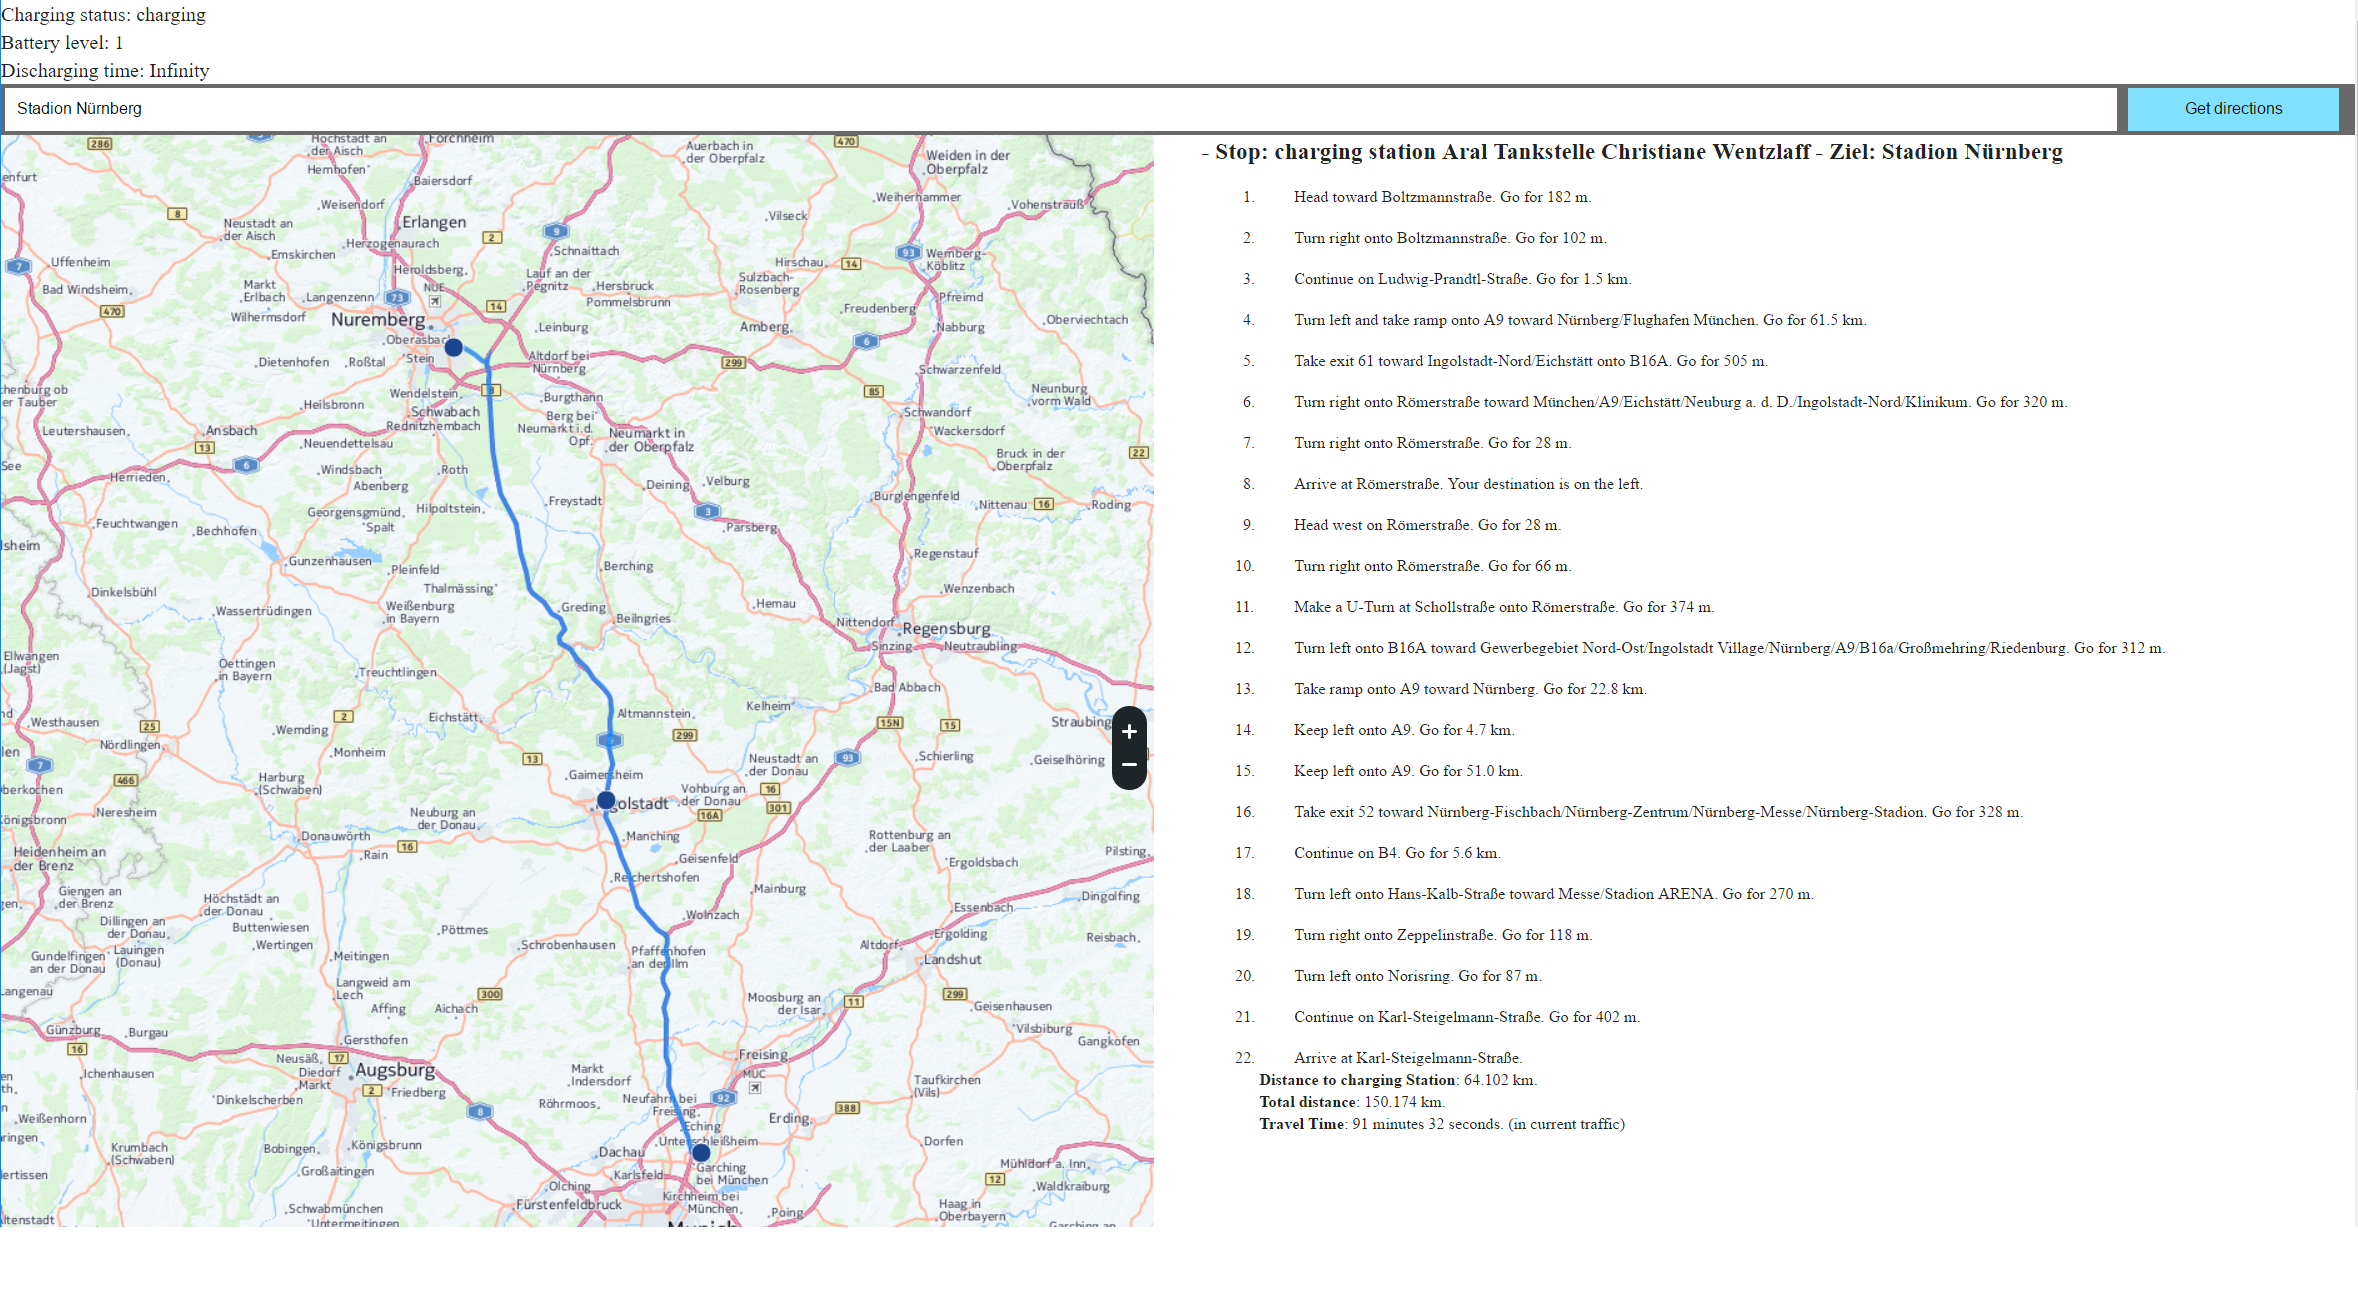
\includegraphics[width=0.46\textwidth]{user_interface}
\caption{User Interface}
\end{figure}

On the left side is the map and the calculated route displayed, in this case from TU Munich to a stadium in Nuremberg, with one charging stop in the middle. At the top is further information about the battery status, for example the charging status and the battery level. On the right side is additional trip information, it is only displayed to show the commands which will then be spoken out by text to speech. These should not be displayed in a later version. On the bottom of the left side is further information about the trip like the total travel time and total distance. 


\subsection{Markup}

As it is the case for the Simulation Manager Interface, the .arkup needed to display the user interface is kept minimalistic. At the top are some div elements to display the battery status of the device. In this case, it is the battery level of the computer it is running on to show its charging status, the battery level and the time till it is fully discharged. If it cannot be read, it will display ``charging state unknown''.

\begin{minted}{html}
<!DOCTYPE html>

<html>
<head>
[...]
</head>

<body>
<div id="charging">(charging state unknown)</div>
<div id="level">(battery level unknown)</div>
<div id="dischargingTime">(discharging time unknown)</div>
<div id="chatbox"></div>
<button onclick="setButtonPressed();">Try it</button>
</div>

<div id="map" style="position:absolute; width:49%; height:100%; background:grey" ></div>
<div id="panel" style="position:absolute; width:49%; left:51%; height:100%; background:inherit" ></div>
[...]
\end{minted}

Below that are two div elements one to display the map and another one to display the panel. All the rest is in JavaScript.

\begin{minted}{html}
<head>
    <meta name="viewport" content="initial-scale=1.0, width=device-width" />

    <link rel="stylesheet" type="text/css" href=".../mapsjs-ui.css" />

    <script type="text/javascript" src=".../mapsjs-core.js"></script>
    <script type="text/javascript" src=".../mapsjs-service.js"></script>
    <script type="text/javascript" src=".../mapsjs-ui.js"></script>
    <script type="text/javascript" src=".../mapsjs-mapevents.js"></script>

    <style type="text/css">
        .directions li span.arrow {
            display:inline-block;
            min-width:28px;
            min-height:28px;
            background-position:0px;
            background-image: url("../img/arrows.png");
            position:relative;
            top:8px;
        }
        .directions li span.depart  {
            background-position:-28px;
        }
        .directions li span.rightUTurn  {
            background-position:-56px;
        }
        .directions li span.leftUTurn  {
            background-position:-84px;
        }
        .directions li span.rightFork  {
            background-position:-112px;
        }
        [...]
\end{minted}

For alignment css is used which is embedded in the head of the html file.

\subsection{Initialization}

\begin{minted}{javascript}
<script type="text/javascript" charset="UTF-8">
    window.onload = function () {
        function updateBatteryStatus(battery) {
            document.querySelector('#charging').textContent = battery.charging ? 'charging' : 'not charging';
            document.querySelector('#level').textContent = battery.level;
            document.querySelector('#dischargingTime').textContent = battery.dischargingTime / 60;
        }

        navigator.getBattery().then(function(battery) {
            // Update the battery status initially when
            // the promise resolves
            updateBatteryStatus(battery);

            // .. and for any subsequent updates.
            battery.onchargingchange = function () {
                updateBatteryStatus(battery);
            };

            battery.onlevelchange = function () {
                updateBatteryStatus(battery);
            };

            battery.ondischargingtimechange = function () {
                updateBatteryStatus(battery);
            };
        });
    };
\end{minted}

First, the battery panel is initiated and set, it will then automatically do subsequent updates. 


\subsection{Route calculation}

As soon as the backend has resolved the locations for optimal charging stops, they can be send as a list to Here Maps to get an optimal route from start \texttt{waypoint0} over potential charging stops \texttt{waypoint1} to destination \texttt{waypoint2}. The number of waypoints is not directly limited and can vary. Additional parameters such as avoiding certain areas, such as a city center, or setting the number of alternative routes can be configured. For a full documentation, have a look here \cite{driver-13}.

\begin{minted}{javascript}
function calculateRouteFromAtoB(platform) {
    var router = platform.getRoutingService(),
        routeRequestParams = {
            mode: 'fastest;car',
            representation: 'display',
            routeattributes: 'waypoints,summary,shape,legs',
            maneuverattributes: 'direction,action',

            // TU Munich
            waypoint0: '48.2626,11.6679',

            // Aral Petriol Station
            waypoint1: '48.7752,11.4595',

            // Stadion Nuremberg
            waypoint2: '49.4268,11.1255'
        };

    router.calculateRoute(
        routeRequestParams,
        onSuccess,
        onError
    );
}
\end{minted}

When the routing API was successful and gives a response, this function will be called. It then calls the different functions and hands over the route element to add the calculated route to the map, highlighting the waypoints and adding direction commands to a list. 

\begin{minted}{javascript}
function onSuccess(result) {

    var route = result.response.route[0];

    /*
     * The styling of the route response on the map is
     * entirely under the developer's control.
     *
     * A representative styling can be found the full
     * JS + HTML code of this example in the functions
     * below:
     */

    addRouteShapeToMap(route);
    addManueversToMap(route);

    addWaypointsToPanel(route.waypoint);
    addManueversToPanel(route);
    addSummaryToPanel(route);

    // ...
}

\end{minted}


\subsection{Route response}

\begin{figure}[htp]
\centering
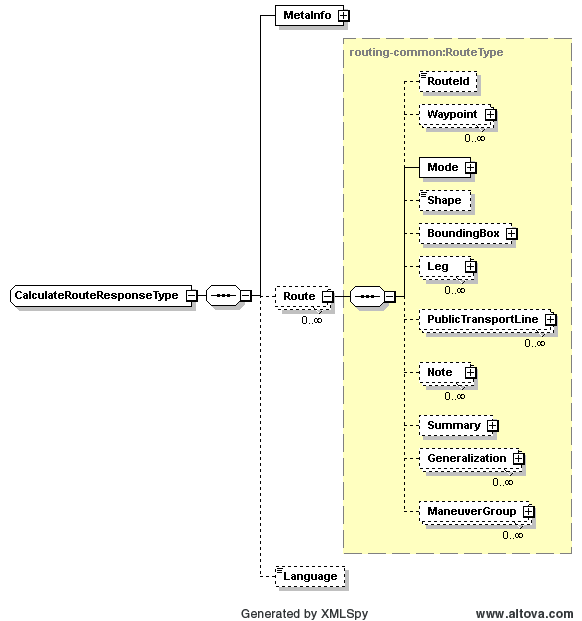
\includegraphics[width=0.46\textwidth]{route_response}
\caption{CalculateRouteResponseType \cite{driver-14}}
\end{figure}

As displayed in figure 1, the route response contains, besides meta info and information about language, the information set for the route. The route itself is stored in a route element, which can appear more than once depending on how many routes were calculated. 


\subsection{Summary Panel}

Here, further trip information is added to the panel which could also be extended to e.g. trip costs or energy used.

\begin{minted}{javascript}
function addSummaryToPanel(route){
    var summary = route.summary
    var summaryDiv = document.createElement('div'),
        content = '';
    var sum = [];

    sum[0] = 0;

    for (var i = 0;  i < route.leg.length; i += 1) {
        for (var j = 0;  j < route.leg[i].maneuver.length; j += 1) {
            sum[i]= sum[i] + route.leg[i].maneuver[j].length
        }
    }

    content += '<b>Distance to charging Station</b>: '+ sum[0]/1000 + ' km. <br/>';
    content += '<b>Total distance</b>: ' + summary.distance/1000  + ' km. <br/>';
    content += '<b>Travel Time</b>: ' + summary.travelTime.toMMSS() + ' (in current traffic)';

    summaryDiv.style.fontSize = 'small';
    summaryDiv.style.marginLeft ='5%';
    summaryDiv.style.marginRight ='5%';
    summaryDiv.innerHTML = content;

    routeInstructionsContainer.appendChild(summaryDiv);
}
\end{minted}

Further information about the trip is added to the panel here. For example, direction commands which could be used for text to speech. In the prototype, they are displayed to show the commands but later on they should not be displayed since it is distracting.

\begin{minted}{javascript}
function addManueversToPanel(route) {

    var nodeOL = document.createElement('ol'), i, j;

    nodeOL.style.fontSize = 'small';
    nodeOL.style.marginLeft ='5%';
    nodeOL.style.marginRight ='5%';
    nodeOL.className = 'directions';

    // Add a marker for each maneuver
    for (i = 0;  i < route.leg.length; i += 1) {
        for (j = 0;  j < route.leg[i].maneuver.length; j += 1) {

            // Get the next maneuver.
            maneuver = route.leg[i].maneuver[j];

            var li = document.createElement('li'),
              spanArrow = document.createElement('span'),
              spanInstruction = document.createElement('span');

            spanArrow.className = 'arrow '  + maneuver.action;
            spanInstruction.innerHTML = maneuver.instruction;
            li.appendChild(spanArrow);
            li.appendChild(spanInstruction);

            nodeOL.appendChild(li);
        }
    }

    routeInstructionsContainer.appendChild(nodeOL);
}
\end{minted}

\begin{minted}{javascript}
Number.prototype.toMMSS = function () {
    return Math.floor(this / 60) + ' minutes ' + (this % 60)  + ' seconds.';
}
\end{minted}

This function can open and display an information bubble at a geo position, for example information about the queue times at a charging stop provided by the backend. Furthermore, a notification can be raised for example if the energy consumption is too high or the battery is running low. 


\subsection{Notification Message}

\begin{minted}{javascript}
function openBubble(position, text){
    if(!bubble){
        bubble = new H.ui.InfoBubble(
            position,
            // The FO property holds the province name.
            {content: text});
        ui.addBubble(bubble);
    } else {
        bubble.setPosition(position);
        bubble.setContent(text);
        bubble.open();
    }
}
\end{minted}

\subsection{Adding the Route and the Waypoints to the Map}

Here, a series of \texttt{H.map.Marker} points from the route is created and added to the map. Furthermore, all the manuevers are then added to be displayed on the map.

\begin{minted}{javascript}
function addRouteShapeToMap(route){

    var strip = new H.geo.Strip(),
        routeShape = route.shape,
        polyline;

    routeShape.forEach(function(point) {
        var parts = point.split(',');
        strip.pushLatLngAlt(parts[0], parts[1]);
    });

    polyline = new H.map.Polyline(strip, {
        style: {
            lineWidth: 4,
            strokeColor: 'rgba(0, 128, 255, 0.7)'
        }
    });

    // Add the polyline to the map
    map.addObject(polyline);

    // And zoom to its bounding rectangle
    map.setViewBounds(polyline.getBounds(), true);
}
\end{minted}


\begin{minted}{javascript}
function addManueversToMap(route){
    var svgMarkup = '<svg width="18" height="18" ' +
            'xmlns="http://www.w3.org/2000/svg">' +
            '<circle cx="8" cy="8" r="8" ' +
            'fill="#1b468d" stroke="white" stroke-width="1"/>' +
            '</svg>',
        dotIcon = new H.map.Icon(svgMarkup, {anchor: {x:8, y:8}}),
        group = new  H.map.Group(),
        i,
        j;

    var marker1 =  new H.map.Marker({
            lat: 48.2626,
            lng: 11.6679} ,
        {icon: dotIcon});
    group.addObject(marker1);

    var marker2 =  new H.map.Marker({
            lat: 48.7752,
            lng: 11.459} ,
        {icon: dotIcon});
    group.addObject(marker2);

    var marker3 =  new H.map.Marker({
            lat: 49.4268,
            lng: 11.1255} ,
        {icon: dotIcon});
    group.addObject(marker3);

    group.addEventListener('tap', function (evt) {
        map.setCenter(evt.target.getPosition());
        openBubble(
            evt.target.getPosition(),
            evt.target.instruction);
    }, false);

    // Add the maneuvers group to the map
    map.addObject(group);
}
\end{minted}
